\documentclass[12pt, a4paper]{report}
\usepackage[top=1.0in, bottom=1.0in, left=0.8in, right=0.8in]{geometry}
\usepackage{graphicx}
\usepackage{amsmath}
\usepackage{listings}
\usepackage{fancyvrb}

 	
\title{\textbf{EE2703 : Applied Programming Lab \\ Assignment 8 \\ The Digital Fourier Transform}} 
\author{Aditya Nanda Kishore\\ EE20B062} 

\date{\today} % Date for the report

	
\begin{document}
		
\maketitle
\section*{Introduction}
In this assignment, we are going to explore the Discrete Fourier Transform(DFT)  of various signals using \textbf{NumPy} commands
\section*{Importing Necessary Libraries}
\begin{Verbatim}

import numpy as np
import matplotlib.pyplot as plt 
\end{Verbatim}

\section*{DFT spectrum function}
We first define a dictionary of functions, whose keys are strings and values corresponding are the actual mathematical functions defined using lambda function

\begin{Verbatim}
func_list = {'sin(5x)': lambda x : np.sin(5*x),
'(1+0.1cost)*cos(10t)': lambda x : (1+0.1*np.cos(x))*np.cos(10*x), 
'cos^3' : lambda x : np.cos(x)**3,
'sin^3' : lambda x : np.sin(x)**3,
'fm' : lambda x : np.cos(20*x+5*np.cos(x)),
'gauss' : lambda x : np.exp(-x**2/2) }
\end{Verbatim}

Since this assignment only asks us to plot the transform function for various functions with different time arrays and sampling rates, I have created a spectrum function to make my job easier. Our function's arguments are
\begin{itemize}
	\item \textbf{func}- A String which maps to the required function in the dictionary defined above.
	\item \textbf{start}- Start of the time array.
	\item \textbf{end}- End of the time array.
	\item \textbf{N}- Sampling Rate. This is the number of samples of the time , frequencies and  function in both time and frequency domain.This has to be varied accordingly for better accuracy.
	\item \textbf{w} - Frequency limit for frequency domain. This is later modified into an array of frequencies on which our plot is plotted.
	\item \textbf{phase-split-plot}- A boolean. If False, it has to plot the phase plot in red dots.
	\item \textbf{magnitude-split-plot} and \textbf{mag-min}- A boolean and a number. If True, It has to plot green dots in the phase plot at the points wherever magnitude is greater than \textit{mag-min}.If false, It only plots the red dots as above.
	\item \textbf{xlim}- Limits for the x-axis in frequency domain
	\item \textbf{plot-name}- String that sets the title of the plot
	\item \textbf{fig-name}- Saves our final plot.png as this string.
\end{itemize}

We write the code for the same using \textbf{numpy.fft.fft} function. We define a time array and map a function to the time array. Then, the \textbf{numpy.fft.fft} maps it to frequency domain by finding it's fourier transform. But we have to take care of magnitude and phase plots by making a few modifications in the arguments of the function like
\begin{itemize}
	\item Peaks need not be present at where we expect them to be. This has to be fixed by \textbf{fftshift} function.
	\item Peaks may have a different magnitude from what we expect. This is because of the scaling up of the fourier transform by a certain number.
	\item Phase at peaks may vary.
\end{itemize}

These can be fixed by choosing appropriately scaled Transform function while plotting as well as choosing proper time arrays and sampling rate.

So, the function would look something like this
\begin{Verbatim}
def spectrum(func,start, end, N, w,mag_plot, magnitude_split_plot, 
phase_split_plot, mag_min, xlim, plot_name, fig_name):
    t= np.linspace(start,end, N+1)[:-1]
    w= np.linspace(-w,w,N+1)[:-1]
    y= func_list[func](t)
    if func == 'gauss' :
        Y = np.fft.fftshift(np.fft.fft(y))/N
        Y = Y *  np.sqrt(2*np.pi)/max(Y) 
    else:
        Y= np.fft.fftshift(np.fft.fft(y))/N
    plt.figure()
    plt.subplot(2,1,1)
    plt.plot(w,abs(Y), lw = 2)
    plt.xlim([-xlim, xlim])
    plt.ylabel(r"$|Y|$",size=16)
    plt.title(plot_name)
    plt.grid(True)
    plt.subplot(2,1,2)
    if phase_split_plot == False:
        plt.plot(w,np.angle(Y),'ro',lw=2)
    if (magnitude_split_plot == True):
        ii= np.where(abs(Y)>mag_min)
        plt.plot(w[ii],np.angle(Y[ii]),'go',lw=2)
    plt.xlim([-xlim, xlim])
    plt.ylim([-2, 2])
    plt.ylabel(r"Phase of $Y$",size=16)
    plt.xlabel(r"$k$",size=16)
    plt.grid(True)
    plt.savefig(fig_name)
    plt.show()
    return Y,w

\end{Verbatim}

In further sections, we are going to use this function with changing arguments again and again to get required plots.
\section*{DFT of a sinusoid}

Now Let's consider a sinusoid function
\begin{equation}
	f(x) = sin(5x) = \frac{e^{j5x} - e^{-j5x}}{2j}
\end{equation}
The fourier transform of this function is 
\begin{equation}
	\mathcal{F}(f(x))(\omega) = \frac{\delta(\omega-5) -  \delta(\omega+5)}{2j}
\end{equation}

For sinusoid, let's take a sampling rate of 128 and time array goes from $[0 ,2\pi)$. 
\begin{figure}[!tbh]
   	\centering
   	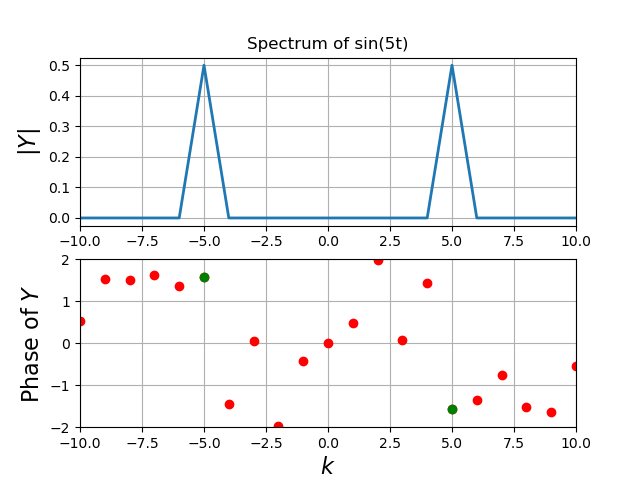
\includegraphics[scale=0.8]{Q1a.png}
 \end{figure} 
 
 \section*{Amplitude Modulation}
 Let's consider a function
 \begin{equation}
	f(x) = (1+0.1cosx)cos(10x)
\end{equation}
 For this , we need a higher sampling rate as peaks are closer and transform changes rapidly.We take it to be 512.
 \begin{figure}[!tbh]
   	\centering
   	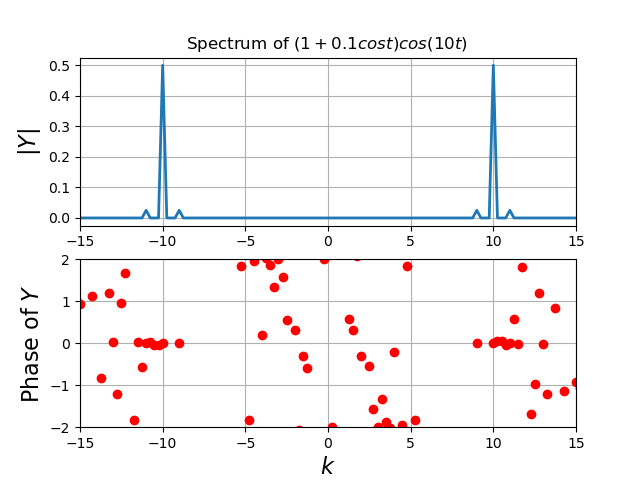
\includegraphics[scale=0.8]{Q1b.png}
 \end{figure} 
 \newpage
 \section*{DFT of Cubic Sinusoids}
 \newline
 Given the functions $sin^3x$ and $cos^3x$.We know that,
 \newline
 \begin{equation}
 	sin^3x = \frac{3sinx-sin3x}{4}
 \end{equation}
 \begin{equation}
 	cos^3x = \frac{cos3x+3cosx}{4}
 \end{equation}
 So, We expect two peaks at frequencies = 1 and 3 and phase difference to be $\pi$ for $sin^3x$ at peaks and phase to be zero at peaks for $cos^3x$.
 Using $N = 512$ for both, we would get


\end{Verbatim}

 
 \begin{figure}[!tbh]
   	\centering
   	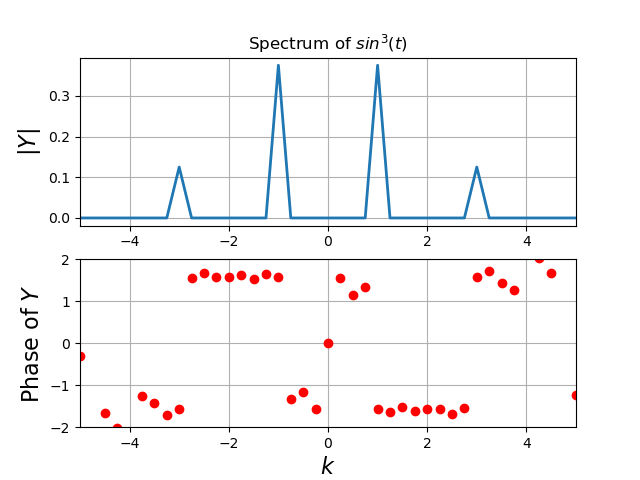
\includegraphics[scale=0.7]{Q2a.png}
 \end{figure} 
 
 \begin{figure}[!tbh]
   	\centering
   	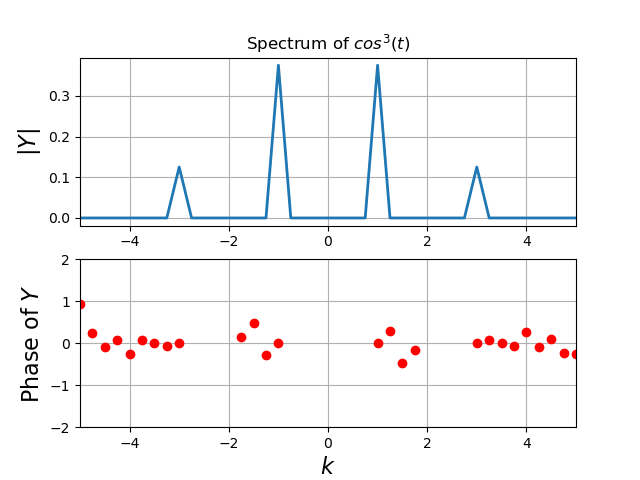
\includegraphics[scale=0.7]{Q2b.png}
 \end{figure} 
 
 \newpage

 \section*{Frequency Modulation}
  For frequency Modulation, we will consider the function $cos(20t+5cos(t))$. For this we can't take a low N as the energy in the sidebands of the peaks is comparable to the signal. If we take time from $[-32\pi, 32\pi)$ and $N= 16384$ and using the same spectrum function as above, we get
  
   \begin{figure}[!tbh]
   	\centering
   	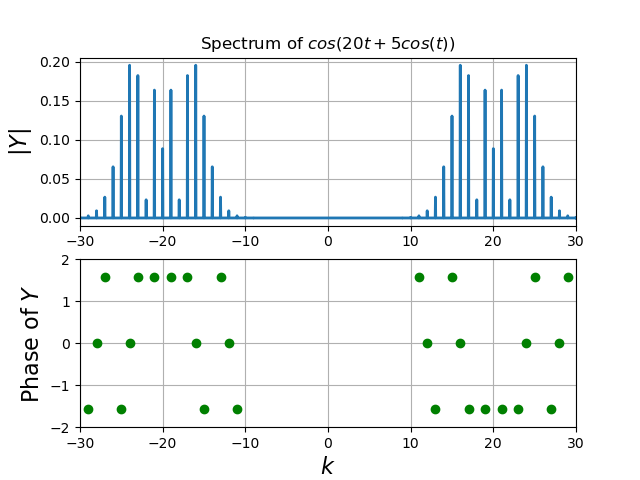
\includegraphics[scale=0.95]{Q3.png}
 \end{figure} 
 \newpage
 \section*{Gaussian Distribution}
 This is a special case. Frequency Transform of a gaussian series is also a scaled gaussian function.It is also not "bandlimited" in frequency, which means the spectrum that we are gonna depends on the $\omega_{lim}$ we choose and also it doesn't decay even for larger frequencies.Let's first analyse the fourier transform of a guassian.
\newline
Fourier Transform of the given CT signal $e^{-t^2/2}$ is given by,
\begin{equation}
\(\int_{-\infty}^{\infty} e^{-t^2/2} e^{-jwt}\,dt\)  = \frac{1}{\sqrt{2\pi}}e^{-\omega^2/2}
\end{equation}

Clearly, It is real. So, The phase plot should be at zero for all $\omega$ and I normalised the Y for Guassian to avoid confusion. The fourier transform's properties still remain the same irrespective of the normalising factor, so it's valid. The only thing we have to take care of now is error.We have to play around with T and N. For that I referred this pdf
\newline

https://nicholasdwork.com/tutorials/approxDFT.pdf
\newline
We can now write CTFT as 
\begin{equation}
X(\omega) = \(\int_{-T/2}^{T/2} x(t) e^{-jwt}\,dt\)
\end{equation}
which as Reimann sum can be expressed using small steps $\Delta t = T/N$ as 
\begin{equation}
X(\omega) = \frac{\Delta t }{2\pi}\[ \sum_{n=-N/2}^{N/2 - 1} x(n \Delta t) e^{-j\omega n \Delta t}  \]
\end{equation}
Now on substituting $\Delta \omega = 2\pi / T$ and rearranging terms , we will get
\begin{equation}
X(k \Delta \omega) = \frac{\Delta t }{2\pi}\[ \sum_{n=-N/2}^{N/2 - 1} x(n \Delta t) e^{-j \frac{2\pi}{N} nk }  \]
\end{equation}
\begin{equation}
X(k \Delta \omega) = \frac{\Delta t }{2\pi}DFT(x(n \Delta t)}
\end{equation}
So for improving accuracy, We have to make T larger as LHS becomes closer to actual function on doing that and also We have to increase N , so that Higher changes in the function are not ignored. Hence, We have to keep increasing T and N till we get $ \epsilon_{max} < 10^{-3}$. If we start with T = $2\pi$ and N = 128, we would get an error of $\epsilon_{max}  = 0.002597659954699405 $, which is greater than 0.001. We can also see that phase is always zero.
 \begin{figure}[!tbh]
   	\centering
   	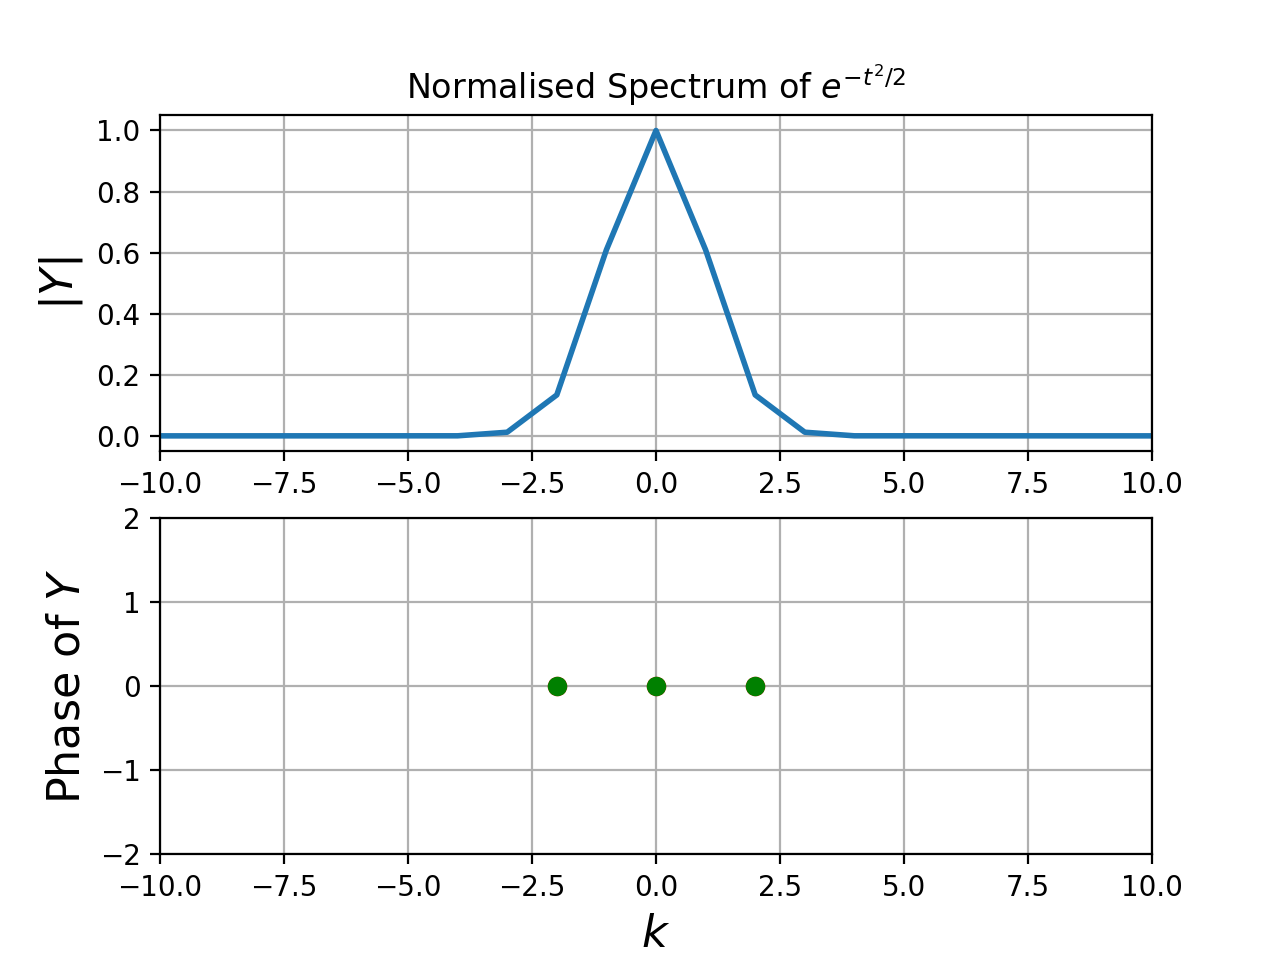
\includegraphics[scale=0.7]{Q4a.png}
	\caption{T = $2\pi$ , N = 128, $\epsilon_{max}  = 0.002597659954699405 $}
 \end{figure} 
\newline
So, we have to double T and N.
 \begin{figure}[!tbh]
   	\centering
   	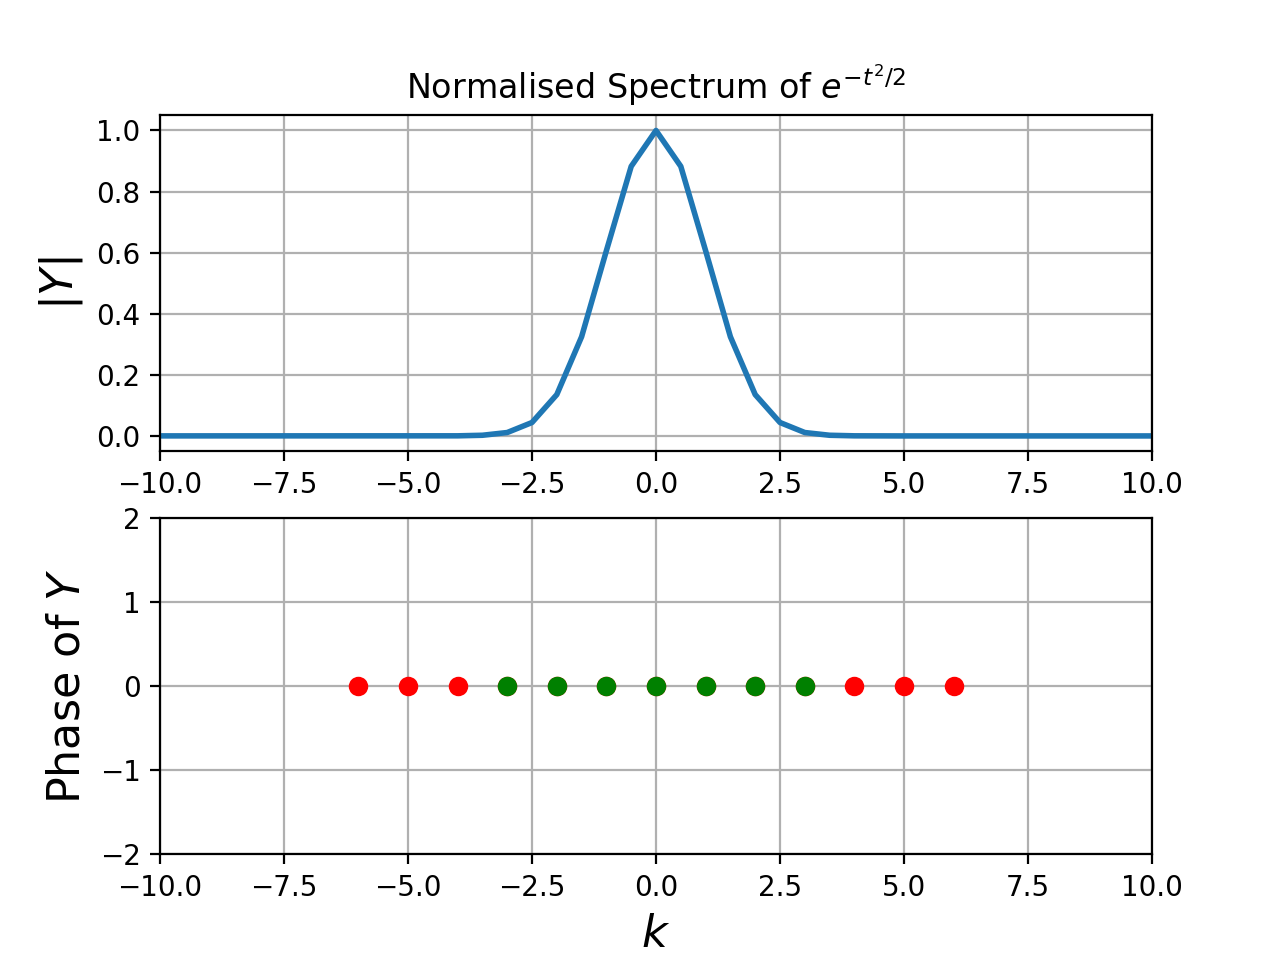
\includegraphics[scale=0.7]{Q4b.png}
	\caption{T = $4\pi$ , N = 256 , $\epsilon_{max}  = 6.27631169258791 * 10^{-10} $}
 \end{figure} 
 \newpage
 As we can see, Error has been decreased by a lot but the curve is not yet smooth.We can make it smoother by increasing T and N further
 \begin{figure}[!tbh]
   	\centering
   	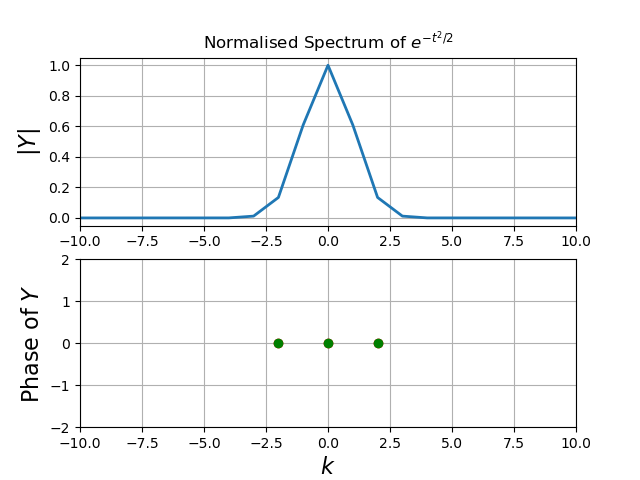
\includegraphics[scale=0.7]{Q4.png}
	\caption{T = $16\pi$ , N = 1024 , $\epsilon_{max}  = 3.8582503464623026 * 10 ^{-16} $}
 \end{figure} 
 \newpage
 \section*{Conclusion}
 \begin{itemize}
 	\item NumPy's \textbf{fft} library has great tools to help us understand the fourier transform better. We can also understand how python works through the fourier transform and how can we improve code's accuracy using \textbf{fftshift}.
	\item DFT's of various sinusoids gave us an idea of where peaks lie and how the phase of peaks should vary. We also examined AM and FM signals to understand how N and T can affect the transform plot.
	\item I also learnt how to use time ranges and sampling improve the accuracy of fourier transform of a discretised continuous time signal.
 \end{itemize}
\end{document}

